%\documentclass[conference,draft]{IEEEtran}
\documentclass[conference,man]{IEEEtran}
\usepackage{ifpdf}
\usepackage[latin1]{inputenc}
\usepackage{cite}
\usepackage[pdftex]{graphicx}
\graphicspath{{.}{images/}} 
\DeclareGraphicsExtensions{.pdf,.jpeg,.png,.jpg}
\usepackage[cmex10]{amsmath}
\usepackage{url}

% correct bad hyphenation here
\hyphenation{op-tical net-works semi-conduc-tor}


\begin{document}
%Encapsulates the theme - should be relevant and precise
\title{Intrusion Detection of a WSN\\Over the Air Update Protocol}

\author{
	\IEEEauthorblockN{	A S M Ashraful Alam, Email: aalam@cs.otago.ac.nz \\
		 and
		 				David Eyers, Email: dme@cs.otago.ac.nz
					}
	\IEEEauthorblockA{Department of Computer Science, University of Otago,
	 					Dunedin , New Zealand	}
}

%\author{
%		\IEEEauthorblockN{	A S M Ashraful Alam\IEEEauthorrefmark{1} and
%							David Eyers\IEEEauthorrefmark{2}
%						}
%	\IEEEauthorblockA{\IEEEauthorrefmark{1}Department of Computer Science, University of Otago, New Zealand, Email: aalam@cs.otago.ac.nz} %Telephone: + 64 (3) 479 8498
%	\IEEEauthorblockA{\IEEEauthorrefmark{2}Department of Computer Science, University of Otago, New Zealand, Email: dme@cs.otago.ac.nz} %Telephone: + 64 (3) 479 5749		 	
%}

\maketitle

\begin{abstract}
%%Write your abstract at the beginning [May be when I have some result]
%%Must have the context; what is the specific issue; what is the research question
%%Why is the question important in this context?
%%Mini version ->	Trailer	of a movie->	
%% These are the things I've found out and it shows a promise for ...
%% What is the method for doing this - in 1 sentence.

%%Relevance of the research question - "So What, who cares?" - must nail down this question

A Wireless Sensor Network (WSN) works in a way that forms an autonomous network and works towards a common goal of sensing and monitoring some phenomena in a unified fashion. 
However, the programmes that run on the sensors might require updating because of changes in requirements, routines, protocols and so on. 
It is not easy to round up all the deployed sensors in order to reprogramme them. 
Hence, the idea of reprogramming over the air (OTA) using the ongoing network transmission came up; several protocols have been developed for this purpose. 
Each protocol has its own suitability depending on the context and scenario.
Deluge is a protocol that allows us to reprogramme over the network. 
The ease of reprogramming opens a backdoor to a potential intruder who can abuse the protocol by injecting a malicious program. 
The design of Deluge do not cater for the intruder's activity; as a result, it is not possible to detect if the update was a legitimate one or not. 
The method we propose analyses the timing of update of each of the sensors in the network and computes a `Intrusion Warning Score' through an algorithmic function to indicate a possible intrusion i.e. a probable illegitimate update. 
%It might be important to avoid readers interpreting the score as an indication of actual intrusion, as opposed to potential intrusion.

\end{abstract}

%\IEEEpeerreviewmaketitle



\section{Introduction}
\label{sec:intro}


%What is WSN?
The idea of Wireless Sensor Network (WSN) has been prevailing for a while, but it has been made a reality only in last two decades. 
The technology has attracted great attention in recent years due to significant advances in wireless and mobile communication technologies. 
One of the main driving force behind quick evolution of WSN is its cost-worthiness and flexibility in deployment.  
The sensors, called the nodes or motes, are generally self-powered, wireless, networked sensing devices with inbuilt limited processing hardware.    
The manager node, which is also called a sink or base station generally has long-lasting power and probably, remain connected to a workstation with greater processing capability. 
Motes and sinks together dynamically form an autonomous networked environment where all sensor nodes within range and sharing the same radio channel and protocols take part.
In such a conventional WSN, data exchange takes place only locally using a autonomous relay mechanism that does not require any routing table to be able to do so. 
A WSN is ultimately employed for sensing and/or detecting certain physical phenomena, on which basic processing is performed at the individual mote, the processed information is relayed back to a computing device  through the sink for further processing.
WSNs are generally deployed for long-term monitoring at scales and resolutions that are difficult to manage. 
They may necessitate reprogramming after deployment to accommodate alteration in the environment, sensing applications, or scientific requirements \cite{ISI:000253439700120}.

%Where does WSN Stand in the development evolution?
Advances in semiconductors and embedded processors initiated the development of sensors with computational capability. 
%The advancement in wireless and mobile communication technology made it possible to come up with a WSN theme.
Conventionally, sensors were built using micro-electro mechanical systems (MEMS) or CMOS or LED technology, based on the purpose and property to sense. 
Today, nano-particles are also used for tiny sized sensors.
It is now possible to combine a wireless radio transceiver with a microprocessor, memory, and other micro-electro-mechanical sensors into a tiny device.
These tiny sensors have advantage of being energy friendly and are deployed in environments with limited power and space.
The WSN evolved from the distributed sensor network programme of the DARPA project and is still evolving with newer and smarter ideas such as integrated RFID-enabled WSN with inkjet-printed electronics on paper substrates,  distributed WSN to tackle reliability, in-network processing to reduce communication cost \cite{5498900}. 
There are other evolving areas like contention and schedule-based energy efficient medium access schemes, cognitive routing methodologies, cross-layer protocols, combining medium access control with routing functionality, security-conscious WSN,  deployment of WSN within aircraft to replace  wired infrastructure and so on.
Today, WSN is developed around an IEEE standard that specifies lower network layers (i.e., MAC layer and physical layer) of a wireless network which focuses on low-cost, low-speed ubiquitous communication between devices \cite{893287}.
%http://standards.ieee.org/about/get/802/802.15.html
%802: Overview & Architecture		http://www.techstreet.com/ieee/products/1850309
%802.1: Bridging & Management
%802.2: Logical Link Control
%802.3: Ethernet
%802.11: Wireless LANs
%802.15: Wireless PANs
%802.16: Broadband Wireless MANs
%802.17: Resilient Packet Rings
%802.20: Mobile Broadband Wireless Access
%802.21: Media Independent Handover Services
%802.22: Wireless Regional Area Networks

WSNs operate unattended over long period of time that may range from months to years.
There is very little control over the sensors once they are deployed.
Changes in the environment and purpose over time affects the operations of the sensors. 
This necessitates reprogramming of the sensors to suit the evolving requirements and also to enable bug fixes after deployment.
The scale and embedded nature of sensors make it impossible to collect every piece of sensors, reprogram them and then redeploy again. 
Network code propagation using data dissemination protocols promises a suitable solution to this problem.


%Why are we interested in WSN? How does that link to security?
The technology promises huge potential for future commercial applications. 
Enormous prospect of WSN has attracted many academics to be engaged in relevant research. 
The technology is still evolving with greater promises of being integrated into even larger scale deployment in the form of Internet of Things (IoT) or dusts.
It is expected to play a critical role in the  computing revolution of cooperating objects and smart embedded devices. 
However, industry adoption is hampered owing to several factors like difficulty in programming, security issues, integration with other systems and business processes and so on. 
Historically, security remains as a neglected part in any implementation process, until there is a major breach. 
One of the main reason why sensor networks has not been widely deployed in industrial systems and safety systems reliably is concerns over security.
Reliability and safety critics and academics have continually expressed that  the security issues in WSN have not been sufficiently addressed and it is not yet secure enough for mission critical employment.
Security is a very important part of system reliability.
Before WSN matures to a point that can be reliably integrated in everyday life, security issues must be adequately addressed. 



WSNs have special vulnerabilities which do not exist in wired networks.
Security mechanism designed for conventional computing systems often are not applicable for WSN.
Even the security techniques like WEP standards for wireless networks cannot be employed in WSN. % because of memory and computing resource constraints.
WSNs are more vulnerable to intrusion attempts and security threats from malicious sources.
The limited resources in terms of memory, computational power and energy, make them easier target. 
The attack targets may range from being on physical sensors, wireless channels, visibility of the network, even  to coordination and self-configuration of the network.

Several approaches to address security issues in WSN have been proposed in recent years. 
They approaches converge on security to ensure reliable data transfer using simple and flexible protocols with high level of confidentiality. 
Because of the resource constraint nature of the motes, security is a vulnerable area to explore.
Lack of suitable computation capability hinders deploying heavy cryptographic measures, wireless nature exposes itself to the adversaries who can easily overcome the barriers to listen to all the traffic and even inject their own packets into the network.
When deployed in a hostile environment, the attackers may have physical or logical access or proximity access capability. 
Threats to security  can be directed to individual motes, towards the network traffic or  a cluster of motes.
A potential adversary may be able to interfere with goals related to security services like authentication, confidentiality, integrity, non-repudiation or even extend to clandestine takeover.
In the event of failure from the expected security services i.e. breach of cryptographic measures, an intrusion detection system (IDS) becomes invaluable.


%On the contrary, these limitations in WSNs can also be utilised as an advantage to protect them from such threats as well.
%The attacker has to employ and utilise own resources because of the limited capability in WSN to incapacitate its functioning.
%How is it related in WSN context?

%What are the security threats to WSN?


%What is intrusion? 
Intrusion is the ability to disrupt or degrade the intended functionality of the network or a part of it; it could be non-intentional or not.
An IDS is able to identify malicious break in attempts  to a trusted environment.
It is directed towards a security mechanism that can detect abnormal behaviour in the network.
A suitable IDS can detect attempt of intentional or unintentional break in events from an insider or outsider party.
However, an IDS does not prevent the break in, but alerts following some predefined procedures in case of a security breach.
Research in WSN security with respect to IDS has lots of potentials for new discovery and implementation.
An IDS architectures for static WSNs has been suggested that watches over the communications in the neighbourhood \cite{roman2006applying}.
Such an IDS is not capable to identify a malicious update that has been effected by an adversary in the WSN.
We propose a novel intrusion detection algorithm that suggest a minor modification of the OTA update protocol by enabling an active message once the update has been completed.
The active message enables a centralised view of a network-wide knowledge  that is processed and analysed to work out a score function according to an algorithmic formula to raise a red flag which could indicate a possible intrusion.



%My Suggested schemes
This work's contributions are two fold. 
We have analyzed 
%AES, RC5 and RC6 in terms of their energy consumption and  memory requirements. 
We have studied how the different  algorithm parameters %(e.g. key size) influence the energy 
consumption. 





%How does WSN work?  -- We are not going to elaborate it here
%What are the main protocols that make it going? ---- We are not going to elaborate it here
%Why a deployed WSN might require updating? 

%How do we do that?

%What is my research question?
%Why the research question is important?


%Context, terminologies to be discussed. Start from the whole story and funnel it down
%This is my research question, 
%Why is the research question important
%Rationale of choosing to research question
%Describe a map of the whole thesis
%
The rest of this report is structured in the following way. In Section \ref{sec:lit}, we discuss the security and intrusion primitives that are talked about in the WSN arena. 
We try to find out what security aspects have not been addressed by the present  security researchers and the reason behind.
In Section \ref{sec:del}, we explain the main concepts of Deluge and its special security measures that have been implemented on Deluge. 
We present design of our proposed algorithm  in Section \ref{sec:deg} and explain how it is connected to the sensor node. 
In Section \ref{sec:imp}, we have explained the experiment methodology and its implementation details.
We then present our evaluation of the experiment in Section \ref{sec:eval}. A few difficulties that we ran into throughout
the development of this experiment are also commented in this section. 
Finally, we conclude our arguments in Section \ref{sec:conc}.
%
%
\section{Related Work / Literature Review} 
\label{sec:lit}
Security is the prime concern in the path to socialising the WSN technology.
Due to its applicability in wide variety of purposes, keeping WSNs secure is a challenging task.
WSNs do not have any session or presentation layer.
Security techniques designed for MANETs are not readily applicable in WSN for its constraints like small processing capability, low battery life, small memory.
various possible attacks on WSNs has been explained by   \cite{roosta2006taxonomy}, \cite{roosta2008attacks}.
On the other hand, WSN security design and analysis suggests many techniques to address them.
Many security schemes for WSN have been proposed targeting two main approaches - using cryptography and using IDS.%to solve the security problems mainly using 
Cryptographic approach actively aims to protect privacy, ensure authenticity, data integrity and confidentiality through use of cryptographic keys and algorithms, policies and procedures.
While symmetric key cryptographic techniques are more efficient in required resources, they suffer from a shortcoming that the key must be shared for being useful. 
However, asymmetric key cryptography is free from this limitation with a greater consumption of resources.
Anomaly detection, on the other hand, is a passive security measure that monitors the behaviour from a observer's point of view and aims to alert a suitable entity for further actions.

Symmetric key cryptographic techniques are useful when both the secret key and the algorithm remains unknown, which can be difficult due to the fact that the WSN is expected to be deployed in exposed environment. Yet, most security schemes in WSN use the technique due to ease of hardware implementation, small computation, power and memory requirements. 
\cite{ISI:000205012800003} recommends Skipjack, MISTY1, and Rijndael to be the most suitable block  ciphers for WSNs, based on the combination of required memory, energy efficiency and intended security strength as the benchmark parameters. In terms of operation mode, pairwise links should use Output Feedback and broadcasts should prefer Coded Block Chain (CBC) mode.
\cite{9783540795902} suggested use of available transceiver chip as resource for hardware based AES encryption in the sensor as it outperforms software implementations of some of the most popular cipher algorithms suitable for WSN.
\cite{5472979} concludes that the lightweight  block cipher proposed by \cite{youssef1996new} achieves good performance, providing  energy efficiency as well as suitable security for sensor nodes  in a WSN in comparison to AES, Skipjack, Puffin, Salsa, Sosemanuk, RC4. 
However, cryptanalysis of the technique by \cite{Heys:1996:CSP} shows that it requires large number of rounds to make it significantly resistant against attacks.
\cite{6216690} found AES to be the most energy-efficient and RC5 to be better than RC6. He also commented that very few security research have been directed towards cryptographic modes of operation in WSN, which might offer interesting insight for certain modes that allow decryption using a decryption block, hence may significantly speed up the execution.
%TinySec is applicable to tinyos 1.x, but you have to change some code to port to T2.  It provides RC5 and SkipJack. Currently, AES is supported by CC2420 chip. You can read the data sheet to start.  Best wishes, Qiyuan Zhang

Asymmetric key cryptography tends to be resource intensive, but has the advantage of private key operation.
It is very suitable in key exchange, digital signature and likewise. 
There are various pubic key cryptographic algorithms like Rabin's Scheme,  RSA, Ntru-encrypt, Elliptic curve cryptography (ECC), Pairing Based Cryptography (PBC) and so on; few of them has been implemented in software and hardware for WSN \cite{ISI:000290947700017}, \cite{ISI:000312683300029}, \cite{ISI:000328624800002}. %Lots of them, \cite{}, \cite{}, \cite{}, \cite{},.
Suitably customised implementations can result in a reduced protocol overhead, less packet transmission and power savings.
ECC and PBC based techniques provide better trade-off  between  key size and security strength than RSA; thus is suggested to be suitable for WSN with advantages like lower computation time, storage space, transmitted data, required energy \cite{Liu:2008:TCL:1371607.1372738}, \cite{Oliveira:2011:TPA:1930560.1931219}.%, \cite{}, \cite{}, \cite{}, \cite{},.
However, asymmetric key cryptography  cannot be used as general purpose scheme, rather to be used for authenticated session establishment, authentication, signature generation and verification, secret key exchange.

IEEE 802.15.4 specification does not require any security implementation. 
Yet, it describes the usage of the AES for either encryption (CTR mode) or authentication (CBC mode) or both (CCM-mode).
Transport Layer Security (TLS) relies on the connection-oriented TCP protocol as transport mechanism.  
%However, many applications used in WSNs run over connection-less UDP protocol.
TLS implementations have been provided in TinyOS; however, Contiki OS still lacks the support. [NEED TO CHECK Contiki ASSERTION]
TinyOS implemented Skipjack algorithm with the CBC mode in TinySec, which has been discarded later on, and support for  hardware based AES-128 encryption has been provided using CC2420 chip.
\cite{ISI:000308844100019}  discovered a (slightly) faster than brute force way to break the AES.  %it would still take trillions of years to recover strong AES keys using the biclique technique, which is a variant of what's known as a meet-in-the-middle cryptographic attack. This method works both from the inputs and outputs of AES towards the middle, reusing partial computation results to speed up the brute-force key search. The technique is designed to reduce the time it takes an attacker to recover the key. 

There are security issues with use of cryptography in WSN due to the nature of the hardware \cite{1710}.
Encryption significantly increases energy and decreases packet throughput.
In many cases, authentication is more desirable than encryption; but encryption is typically the standard method for authentication.
Absence of session and presentation layers complicates the design security protocols.  %Released in September 2007 as part of HART 7 specifications
Moreover, WSNs do not have gateways or switches that can enable monitoring of the information flow.
Hence, in case of failure from cryptographic measures, intrusions need to be detected before or after attackers have succeeded in breaching the WSN. 

Usually an IDS detects suspicious behaviour in the WSN.
IDS may also provide some of the information like identification and location of the intruder, extent of intrusion and so on.
Butun, Morgera, and Sankar authoritatively discussed the constraints and challenges in WSN IDS design \cite{6517052}.
%I may summarise and argue on that 
IDSs in WSN have been suggested using distributed and cooperative architecture. 
Some other IDS also exist that  uses a  hierarchical and centralised approach.
Anomaly based approach works in a distributed manner using support vector machine that minimizes communication overhead while performing in-network anomaly detection propose dby \cite{ISI:000257882502160}.
A standalone rule based approach to detects anomalies at all layers of a network stack in WSN has been suggested \cite{ISI:000232429900067}.
Rule based  techniques rely  monitoring of group of nodes and routing tables for detection \cite{ISI:000298891500099, Chen:2009:NMI:1516241.1516282, 1424814, Strikos_afull}.
Spontaneous watchdog uses the sensor broadcast, density of deployed sensors for its detection \cite{1593102}.
Specification based  IDS has been proposed that relies on data clustering and uses standard deviation from the average inter-cluster distance \cite{Chen:2009:NMI:1516241.1516282, 1424814, Strikos_afull, 4085803}. 
Statistical based anomaly  detection looks for anomalies in routing pattern \cite{4024996}.
Statistical methods that use hidden Markov model focus on the accuracy of the gathered data, rather than the security of the nodes or the links.  \cite{1290173}.
Such a model monitors data arrival process in real time traffic on the nodes, analyses short term dynamic statistics using a multi-level sliding window event storage scheme that works on each node. The detection algorithms performs locally and individual nodes are not aware of the network-wide attacks \cite{1515559}.
Some other statistical based procedure exploits the stability of the neighbourhood information of the WSN nodes depending on average receive power and average packet arrival rate \cite{1512911}.
Game theory based IDS utilise Markov chain for its decision making process can monitor only one of the clusters of the network at a time, which leaves the rest of the network unprotected \cite{1347798}, \cite{Das07preventingdos}, \cite{Reddy:2009:GTA:1607720.1607944}.
Reputation based IDS relies on heuristic ranking algorithms to identify most likely bad nodes in the network.
Such IDSs use high scalable cluster-based hierarchical trust management protocol to effectively identifying the selfish and malicious nodes \cite{6174485}.

Software update in a WSN is a vulnerable process from security point of view.
While cryptography  is an algorithmic  tool designed to verify authenticity and ensure security, IDSs  monitor anomaly in network behaviour  and raises alarm. 
There are other IDSs that initiate  countermeasure process also, in addition to monitoring and raising alarm. 
Cryptography and monitoring both work in collaboration with each other and are intended to ensuring security and protect  against intrusion.
Despite these efforts, WSN passes through a vulnerable phase during the software update process due to the fact that the running operating system and application needs to switch from old version to the new ones and there is a significant increase in traffic owing to software update process.
There are high number of transmitted packets in the network that uses huge network bandwidth, thereby depletes sessor energy.
When a software update in WSN takes place, it replaces the executing embedded operating system and running application as a package.
Cryptographic measures and IDS running in the local sensors are deactivated or unavailable, which open up a vulnerable  window in time when it is easy for an intruder due to the transition.
Therefore, this is a special case from security point of view and must be dealt with specific measures like an additional layer of security measures that must observe the update behaviour. 

%%%%%%%%%%%These MANET IDSs cannot be implemented in WSN ref http://ieeexplore.ieee.org/xpl/articleDetails.jsp?arnumber=6517052
% % Wrong effort {wasted??}
% % IDS has been extensively investigated in MANET and some of the techniques can be implemented suitable in WSN. 
% % In an agent based distributed and collaborative IDS, every node participates in the decision making process. Detection is made by using the means of ``entropy''.  Local IDSs trigger global IDS for collaborative decision making through a majority voting process. \cite (15,33,34)
% % Clustering based / Hierarchical IDSs, only cluster heads (CH) participate in decision making. The scheme is suitable for  clustered MANETs or power supplied sensors only. \cite (35)
% % Both the approaches are not suitable for  WSN because of individual work load would deplete sensor energy.
% % Statistical detection based IDSs uses estimated congestion at intermediate nodes to make decisions and require considerable data processing in order to sift the information, hence is not applicable to WSN. cite{36,37}
% % MANETs.
% % Reputation or trust based IDSs scheme promotes node cooperation through resulting grading system associated with collaborative monitoring of alarm messages from trusted nodes.
% % The neighbourhood watch scheme detects intrusive activity made by the next node on the source route and sends an alarm message to other nodes on its list of trusted neighbours. The scheme is bandwidth and power consuming, cannot be suitable for WSN \cite(16, 39).

%10.1 AES Encryption
%--------------------------------------------------------------------
%The CC2420 chip itself provides AES-128 encryption. The implementation involves loading the security RAM buffers on the CC2420 with the information to be encrypted - this would be the payload of a packet, without the header.  After the payload is encrypted, the microcontroller reads out of the security RAM buffer and concatenates the data with the unencrypted packet header.  This full packet would be uploaded again to the CC2420 TXFIFO buffer and transmitted.  
%Because the CC2420 cannot begin encryption at a particular offset and needs to be written, read, and re-written, use of the AES-128 may be inefficient and will certainly decrease throughput.
%10.2 Authentication
%--------------------------------------------------------------------
%In many cases, authentication is more desirable than encryption. Encryption significantly increases energy and decreases packet throughput, which does not meet some application requirements. A layer could be developed and added toward the bottom of the radio stack that validates neighbors, preventing packets from invalid neighbors from reaching the application layer.  Several proprietary authentication layers have been developed for the CC2420 stack, but so far none are available to the general public.
%A solid authentication layer would most likely involve the use of a neighbor table and 32-bit frame counts to prevent against replay attacks. Once a neighbor is verified and established, the node needs to ensure that future packets are still coming from the same trusted source.  Again, some high speed low energy proprietary methods to accomplish this exist, but encryption is typically the standard method used.
%TinySec is a layer security architecture which was implemented in TinyOS 1.x by Chris Karlof, Naveen Sastry and David Wagner. This implementation was not ported to TinyOS 2.x.
%TinySec provides two different modes: authenticated encryption (TinySec-AE) and authentication only (TinySec-Auth). Encryption is provided by the Skipjack algorithm used with the  CBC mode of operation. Authentication is provided by the CBC mode of operation wich adds a 4-byte tag to the message.

%%%%%%%%%%%%%Notes on Skipjack %%%%%%%%%%%%%%%%%%%%%%%%%%%%%%%
%Skipjack uses an 80-bit key to encrypt or decrypt 64-bit data blocks. It is an unbalanced Feistel network with 32 rounds.[http://csrc.nist.gov/groups/ST/toolkit/documents/skipjack/skipjack.pdf] It was designed to be used in secured phones.
%Cryptanalysis
%Eli Biham and Adi Shamir discovered an attack against 16 of the 32 rounds within one day of declassification,[http://www.cs.technion.ac.il/~biham/Reports/SkipJack/note1.html] and (with Alex Biryukov) extended this to 31 of the 32 rounds (but with an attack only slightly faster than exhaustive search) within months using impossible differential cryptanalysis.[http://www.iacr.org/cryptodb/archive/1999/EUROCRYPT/15920012.pdf]
%A truncated differential attack was also published against 28 rounds of Skipjack cipher.[http://www.eecs.berkeley.edu/~daw/papers/skipjack-talk.ps]
%A claimed attack against the full cipher was published in 2002,[http://csis.bits-pilani.ac.in/faculty/murali/netsec-10/seminar/refs/apoorv2.pdf] but a more recent paper with attack designer as a co-author clarifies that no attack on the full 32 round cipher is known to date.[https://dspace.lboro.ac.uk/dspace-jspui/bitstream/2134/8159/1/kim.pdf]

%%%%%%%%%%%%%Notes on MISTY1 %%%%%%%%%%%%%%%%%%%%%%%%%%%%%%%
%MISTY1 is one of the selected algorithms in the European NESSIE project, and has been among the cryptographic techniques recommended for Japanese government use by CRYPTREC in 2003; however, it was dropped to "candidate" by CRYPTREC revision in 2013.
%MISTY1 is covered by patents, although the algorithm is freely available for academic (non-profit) use in RFC 2994.
%MISTY1 is a Feistel network with a variable number of rounds (any multiple of 4), though 8 are recommended. The cipher operates on 64-bit blocks and has a key size of 128 bits. MISTY1 has an innovative recursive structure; the round function itself uses a 3-round Feistel network. MISTY1 claims to be provably secure against linear and differential cryptanalysis.

% Recently researchers have shown that heterogeneous sensor networks can perform better than homogeneous sensor network. 
%\cite{6785489} proposes a post-deployment pairwise key distribution scheme for two-tier sensor networks that builds a special tree structure for generating the addresses for the nodes in the network, generates pair-wise keys shared with neighbour nodes. The author contends that the scheme has fewer security overheads, uses little memory to store the keys, and has smaller computation overhead, and is strongly resilient against the node capture attack.

%%%%%%%%%%%%%%%%%%%%%%%%%
%%%COMMENT
%%We can also talk about this protocols if space permits
%% Some sensor network applications, such as Tiny Diffusion[8], Maté [12], and TinyDB [17], use concise, high-level virtual code representations to reduce this cost.
%%8 J. S. Heidemann, F. Silva, C. Intanagonwiwat, R. Govindan, D. Estrin, and D. Ganesan. Building efficient wireless sensor networks with low-level naming. In Symposium on Operating Systems Principles, pages 146-159, 2001.
%%12 D. Kotz, C. Newport, and C. Elliott. The mistaken axioms of wireless-network research. Technical Report TR2003-467, Dept. of Computer Science, Dartmouth College, July 2003.
%%17 J. Luo, P. Eugster, and J.-P. Hubaux. Route driven gossip: Probabilistic reliable multicast in ad hoc networks. In Proc. of INFOCOM 2003, 2003.
%%Multi-hop Over-the-Air Programming = T. Stathopoulos, J. Heidemann, and D. Estrin. A remote code update mechanism for wireless sensor networks. Technical report, UCLA, Los Angeles, CA, USA, 2003.
%%Infuse S. S. Kulkarni and M. Arumugam. INFUSE: A TDMA based data dissemination protocol for sensor networks. Technical report, Michigan State Univ., East Lansing, MI, USA, 2004.


%%Existing Gaps in works: 
%Modelling of data/malware propagation over dissemination protocols (especially in mobile sensor networks)
%Reprogramming protocol in mobile WSN
%Performance analysis in mobile scenario[Markov Chain based model, MAC analysis in 802.11, derive throughput of delivery] 


%%Our solution to the secure programming problem leverages authenticated streams, is consistent with the limited resources of a typical sensor node, and can be used to secure existing network programming systems. 
%%Under our scheme, a program binary consists of several code and data segments that are mapped to a series of messages for 
Several network data dissemination protocols have been implemented in different sensor/embedded systems operating systems.
All the OTA software update protocols are targeted at attaining efficiency, throughput and conserve energy.
The  OTA reprogramming systems, in general, do not provide cryptographic protection for source authentication, integrity verification and likewise. 
Limitations of various techniques that can be used in WSN reprogramming has been elaborated in \cite{1127826}. 
The program binary authentication technique using a hash is not very useful in to resource-constrained sensors. 
Deluge has been enhanced to handle security that we have elaborately discussed in section~\ref{sec:del}. 
Deluge uses digital signatures for codes signing and authenticated broadcast scheme. 
It also incorporates digitally signed initial advertisement, which in turn authenticates the following messages in a chained fashion much like the CBC methods used in public key cryptography.
However, we contend that it is possible for a malicious intruder to replicate an authentic image source and advertise new programme version which the motes cannot repudiate. 
Even though,  Deluge incorporates on-chip hardware based AES-128 encryption,
Cryptography cannot completely prevent attacks.%on WSNs confidentiality, authenticity, availability due to resource limitation.
Constrained computational capacity and resources make it possible to compromise the cryptographic measures incorporated in the implemented WSN operating systems.
The other vulnerability of such epidemic protocol is breach at any one point does the job of weakening the whole network for the attacker. 
It is possible for him to appear somewhere in the network, pretend to be an authentic source and disappear after successful transfer of the complete image to only one of the motes in the network. 
The security mechanisms provided by Deluge would be unable to detect the initial breach in such cases and would allow the network to be flooded by a totally new version of the application that performs completely different function \cite{Karlof:2004:TLL:1031495.1031515}.
While the reprogramming protocols are essential for the WSNs, they could act as carriers of rapid spread of malicious code in the network.
Hence, we propose an analytical tool that can have valuable insight into the propagation characteristics of OTA reprogramming protocol. 
The tool should be flexible for comparative studies of different protocols. 

There is no previous works available that targets to secure update process using an IDS.
The security countermeasures available in WSN systems is predominately cryptographic.
None of the well-known WSN operating systems have ever incorporated an IDS due to the reality that such an employment would cut down on the resources, especially power.
An IDS residing on the sensors is ideally need to be avoided by design.

Hence,we propose an IDS that can primarily be applied on OTA protocol.
The technique has been tested successfully on Deluge.
We have exploited services from other existing standard protocols a to gather timing information outside the WSN and then process the timing information for intrusion detection.
Use of timing analysis approach is a new technique in IDS for WSN.
The technique may further be extended for use with broad range of intrusion detection motives specially in WSN and also in MANET.
The technique is centrally controlled, resides outside the WSN, gathers processed information from the sensors in WSN.
However, an IDS with that broad spectrum is out of scope of this paper.
We shall limit ourselves within its application on WSN, specifically on Deluge only.
Before one understands how the IDS works and is able to focus on its  mechanism, one needs some prior knowledge about Deluge and its security techniques.


ADDITIONAL NOTES TO BE INCORPORATED or DISCARDED
% Features, advantages and disadvantages of the protocols.
% Comparison among protocols, similarities and contrasts.

%Limitations of Current Schemes
Most of the solutions are context specific and are vulnerable depending on its application.
The assumptions made on the corresponding threats may be inconsistent with the problem domain and attempts to address unrealistic problems.

%Are you sure that a solution can be found within time available? How do you know?
WSN have limitations in computing resources, memory and physical security. 
Even after stringent security implementation, it cannot overcome security threats and possible security weakness. 
Sensor nodes use wireless communication, which is particularly easy to eavesdrop on. Similarly, an attacker can easily inject malicious messages into the wireless network.\\


\cite{ioannis2007towards} suggests a distributed approach in which nodes do not have a global view, monitor their neighbourhood and collaborate with their nearest neighbours for their normal operational condition, yet can detect an intrusion against blackhole and selective forwarding attacks.
\cite{sen2010efficient} proposes a mechanism based on trust that uses node localisation, density of the WSN, collaborative sensing, cryptographic techniques  and focuses on misbehaviour characterisation and behaviour monitoring to build a `Reputation Table' for each node . However, the mechanism have assumptions about motives of the adversary, symmetric links, nodes  are not compromised or faulty at the time of bootstrapping. 

\cite{Zhu:2007:IHA:1267060.1267062} proposes a guaranteed interleaved hop-by-hop authentication schemes for detection of injected false data immediately when no more than t nodes are compromised, where t is a system design parameter. 




\section{Deluge} % \& Intrusion}
\label{sec:del}

%What are the update technologies available?
%What are the update protocols available?

\subsection{Popular OTA Protocols}
Reprogramming of the sensors in a WSN is one of the most important management task.
Performing the task manually may work out for a small no of sensors, but this is not a scalable idea.
Hence automatic OTA reprogramming of sensors becomes an important issue.
While some of the protocols designed for OTA reprogramming deals with a subset of motes, most others necessarily update the whole network at one go resulting into all motes in the WSN running same version of the software.
The subset reprogramming allows the same WSN to preferentially perform different tasks, which is a convenience and again increases management overhead.
% XNP  [4]	Program	CSMA	One	 \cite{xnp}
% Incremental  [15]	Patch	CSMA	One	No	No  \cite{1381899}
% Trickle  [19]	Script	CSMA	Multi	No	No \cite{ISI:000221664800002}
% Deluge  [13]	Program	CSMA	Multi	No	Yes \cite{1031506}
% MNP  [17]	Program	CSMA	Multi	No	Yes \cite{Kulkarni:2005:MMN:1068511.1069352}
% Sprinkler  [22]	Program	TDMA	Multi	Yes	No \cite{4212092}
% Firecracker  [18]	Program	CSMA	Multi	Yes	No \cite{Levis:2004:FP:1133572.1133589}
In Trickle, which is a well-known OTA update protocol, the motes periodically advertise their own running code version to the neighbours. 
When a neighbour listens to an older version, it disseminates the updated code. 
Trickle addresses single packet dissemination and uses suppression and dynamic adjustment of the broadcast rate to limit transmissions among neighboring nodes.
The Trickle algorithm controls the rate of transfer by suppressing a motes own broadcast  instead of flooding the network \cite{ISI:000221664800002}.% scalable multicast, and wireless broadcast literature
Another OTA update protocol, Multihop Network Programming (MNP) is an enhancement over Trickle or Deluge in a way that is more efficient in image transfer using `pipelining' to enable faster data propagation and also in terms of energy.
MNP handles the problems that occur from message collision and hidden terminal using a greedy approach of sender selection algorithm to guarantee that at a time, there is at most one programme transmitting source  in a neighbourhood. 
MNP  \cite{Kulkarni:2005:MMN:1068511.1069352}.
While the above mentioned reprogramming protocols  are either unsuitable or inefficient in a mobile environment, ReMo does not make any assumptions on the location of nodes and suggests an energy efficient, multihop reprogramming protocol for mobile WSNs.
ReMo is based on a periodic metadata broadcast paradigm whose probability is dynamically adjusted based on neighbour density and pages are transferred out of order based on availability which in turn depends on high potential of code availability, not link quality alone \cite{ISI:000271540300007}.
Comparison of code update completion time of different protocols indicates that while Deluge performs moderately, MNP is the fastest among them.
Typhoon also reliably delivers large objects to all nodes using a combination of spatially-tuned timers, prompt retransmissions, and frequency diversity  and has the benefits of reduced dissemination time and energy consumption by up to three times \cite{liang2008typhoon}.
MOAP-SW allows a subset of the network to be programmed efficiently \cite{Maia20131277}.


\subsection{Deluge Protocol}
%In this section,we describe Deluge protocol.
Deluge is an efficient and reliable protocol for disseminating large data objects, such as program binaries that are larger than sensor memory \cite{1031506}. 
Combining the mechanism with bootloader  allows programming the wireless nodes over the air.
Deluge has been implemented in TinyOS and later ported on Contiki, bothare prominent WSN open source operating systems.
%TinyOScomponent-based operating system and platform targeting wireless sensor networks (WSNs). TinyOS is an embedded operating system written in the nesC programming language as a set of cooperating tasks and processes.
%Contiki is an open source operating system for the Internet of Things. Contiki %connects tiny low-cost, low-power microcontrollers to the Internet. 
The original protocol was implemented at Barkley by Jonathan Hui. % Now in CISCO
The later version Deluge 2.x was implementation at Johns Hopkins notably by Razvan, who is also credited with secure design of the protocol and author of another OTA protocol Typhoon. %  (now at Google).
Deluge, (which is) an improvement over Trickle,  divides the program image into pages that are further split into packets while in transition. 
Instead of nodes autonomously advertising its own version like Trickle, the nodes periodically advertise the newest pages (only the ones changed from prior version) available to send. 
Other nodes then request the required pages following a sequential order \cite{1031506}.

Deluge solves several problems in network programming. 
It deals with larger program image or data objects, mostly much larger than the memory (RAM) available in a sensor.
It works on an environment where node density is variable to the extent that includes assymentric links as well.
It displays reliable behaviour by correcting packets in environment that is characterised by high packet loss rate.
Deluge ensures that all the nodes remain updated with the latest software version.
In cases when a node missed several updates and needs to update its state to the very newest version, it can do so without requiring to go through the missed updates.
The protocol ensures quick propagation of program codes and requires minimum service interruption. 

Deluge displays few prominent characteristics that make it prominent.
It transfers complete binary image when it is necessary to do so. 
It disseminates a program, image from one or more sources to many nodes over multi-hop WSN.
The density aware epidemic property achieves reliability in the unpredictable wireless medium.
The epidemic protocol works on a state machine principle and follows few local rules that ultimately achieves global behaviour.
Deluge allows the sensor to store multiple program images in its flash memory, one of them is identified as golden image which is able to run with minimal support in case of a failure.
Deluge can work in conjunction with a isolated bootloader to switch from running image to a newer one.
The protocol achieves high performance due to its three-phase handshaking technique, robust support for asymmetric links and density aware mechanism that supresses redundant advertise messages and requests. 

To represent large data objects, Deluge splits in into fixed size pages.
Pages are basic data transfer objects which are further split into fixed no of packets for wireless transmission.
Both pages and packets use 16bit CRC for integrity and data correctness.

The deluge mechanism is simple yet interesting. 
Each node periodically advertises its version no and summary of software/data object.
Version no is used to differentiate between updates and is chronologically increased for each subsequent updates.
Nodes in the neighbourhood can determine from this advertisement if any of its neighbours have an old profile. 
Nodes listening to such advertisements suppresses their own advertisement if it has the same version of software; however, if it has a newer version then responds with its object profile.
This is done in a fashion that can be termed as controlled flood.
The nodes with older data object then determines which portion of data it needs updating and requests it from any neighbour it can reach.
It works through a three-phase handshaking (advertise-request-updates) protocol which is helpful in a lossy environment to achieve reliability. 
Node with an old profile requests for the new page and switches to new \textit{receive} mode.
However, the neighbouring nodes which require the update can take advantage by receiving the same page without entering into a contention for requesting. 
The nodes utilise pipelining to increase throughput by working on completed pages before all pages in the image are complete.

A node in \textit{receive} actively requests remaining packets required to complete a page. After making a request, the mote waits for response. However, a node need not be in \textit{receive} mode in order to receive data packets.
Packets needed to complete a certain page are saved without any regard to its state.
A node in \textit{transmission} broadcasts all requested packets from a given page in round-robin order with an aim of achieving fairness.

\subsection{Security of Deluge}
The original Deluge protocol did not consider security of operations.
Security of Deluge was mainly suggested by \cite{1127826} in the form of solution to following problems:
\begin{itemize}
\item	Authentication of program binary ensures that the transferred program image is from its author and has not been forged. This is usually done by signing and verifying the data stream.
\item	Verification of data integrity ensures that the binary was not changed during transit and if there was a change then it is detected by the recipient. 
\item 	System freshness ensures that older programs cannot overwrite the newer ones.
\end{itemize}
Since size of the entire program, page and packets are known before a transmission takes place, the program can be split into messages, each message contains a cryptographic hash of the next message and digitally sign the head of hash message.
It suggested to use a particular implementation of RSA signature and SHA-1 hashes.
However, the RSA signature technique has not been implemented, instead AES-128 based symmetric key has been chosen, as we have mention beforehand. 
Use of hash function that binds later packets is a kind of digital signature by the base-station, and  facilitates authentication \cite{1127826}.
%However, the literature suggested several potential security and performance  improvement of the Deluge protocol.
%Select a linear set of nodes thorugh 


%How does Deluge handle security? 

% title = {Securing the Deluge Network programming system},
% http://www.cs.berkeley.edu/~jwhui/pubs/ipsn06-secureDeluge.pdf

\subsection{Security Vulnerability of Deluge}
Deluge security measures are not conclusive to this assertion that it can completely resent security threats. 
An adversary may employ  the suppression to prevent the update propagation, waste network resources, disrupt the normal operation of code dissemination. 
He may even be able to inject malicious codes to pollute the network and deny intended function.

Advertisements are not authenticated, any node in the WSNs may advertise any message. So an adversary can 
launch several attacks on Deluge by injecting bogus or modified advertisement packets 

%adversary can personate a source to inject an  unexpectable or harmful code image into a WSN

%Forge the version number of a code image in the advertisement packet
%In order to exhaust the energy of a node, a malicious node may continuously request the same pages or unwanted pages from a normal node to trigger the transmission of code data packets.


\section{Design and Implementation}

%Research Question
Is it possible to detect malicious software updates applied using over the air update protocol (especially Deluge) with multihop sensor networks using timing analysis approach?
We hypothesize that it is possible to detect intrusion by analysing the timing of the software update of the motes in WSN.
The pattern generated from the analysis is dependent on relative physical position of the motes and time of update.

We perform a comprehensive evaluation of mote update time.
After a new data object is delivered to the mote and the mote uses the bootloader to start running the new data object is the time we are interested in.
%[You're not being precise about what type of update this is. It's a software update, and the time is the time to complete the verified propagation of that software update. (I think?)]
%using an OTA [Abbreviation should be used first alongside their expansions ... although this one may well occur earlier in the thesis, of course...]
Measurement of the update time has been simulated on different topologies. 
Using different topologies provides us with topological diversity which is at par with the 
randomness that is expected in a real-world WSN deployment.[Some are random, some aren't: I'm not sure that those contexts can be intermixed ...]
Study of different topologies is a structured way of studying such deployments
\label{sec:deg}


\subsection{Identification Requirement}

\subsection{System Design}

The system is aimed at detecting deviation form expected behaviour

Sink starts disseminating new image using Deluge protocol.
Whenever a mote receives full data object, it reboots to the new image and sends a confirmation timing info using AM to Sink.
Sink updates the NDB with timing info, moteID.
IDS builds baseline basing on authentic info.
IDS calculates surprise score using baseline and utility function.
IDS raises alarm using threshold score.

\begin{figure}[btp]
    \centering
    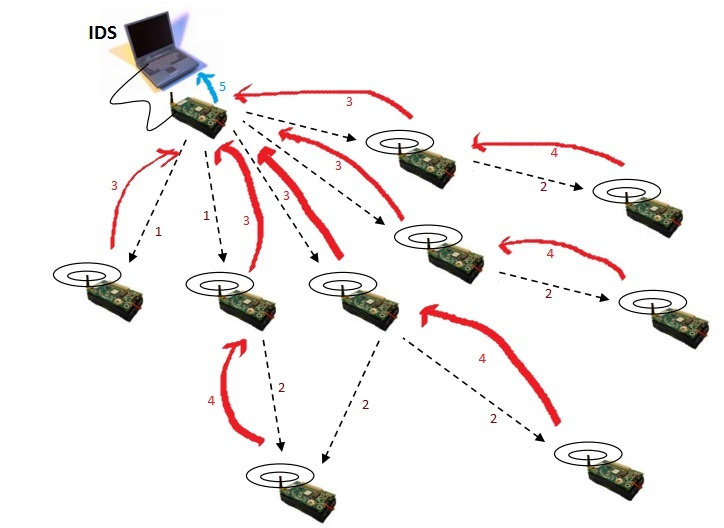
\includegraphics[width=0.5\textwidth]{IDS}
	%\includegraphics[scale=0.5, angle=180]{chick}
    \caption{IDS Modelling}
    \label{fig:ids_model}
\end{figure}


\begin{figure}[btp]
    \centering
    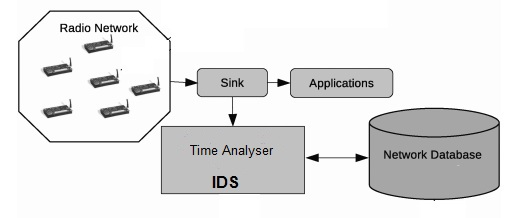
\includegraphics[width=0.5\textwidth]{IDS_fw}	
    \caption{IDS Framework}
    \label{fig:ids_fw}
\end{figure}

Utility Function / Surprise score

\begin{equation}
\label{eqn1} 
f_1 \eq \sum\limits‎_‎{i=0}^{‎n‎} ‎\left( \mu_i - t_i \right)‎‎
\end{equation}

\begin{equation}
\label{eqn2} 
f_2 \eq \sum \limits_‎{i=0}^{‎n‎} \frac{‎\left( \mu_i - t_i \right)‎‎}{\left( \sigma_i + 1 \right)‎‎}
\end{equation}

where, \\
\hspace {2cm} $\mu_i$ - Mean Time at Mote \emphasize{i} \\
\hspace {2cm} $\sigma_i$ - Standard Deviation of  Time at Mote \emphasize{i} \\
\hspace {2cm} $t_i$ - Image Update Time at Mote \emphasize{i} \\
\hspace {2cm} $i$ - Identification of the Mote  \\


\subsection{Assumptions}

A single BS in the WSN
The BS is protected and cannot be compromise
All motes in the WSN are static
We have knowledge about the topology
The software update behaviour in the WSN is transperant to the IDS
The IDS resides externally outside the WSN (not in motes)


\begin{itemize}
	\item	The WSN is of homogeneous nature and works in the same network
	\item	Each of the motes are  connected via wireless to at least another mote
	\item	Whenever possible, there are more than one route to reach each of the motes
	\item	The WSN is static in nature
	\item	Whenever a new image is updated in a mote, it sends a conformation active message to all base stations in the WSN
\end{itemize}

\subsection{Threat Model}

%What are the security aspects it does not handle?
%Why does not it handle them?

Directed towards unauthorised program image to infect the entire WSN.
\begin{itemize}
\item Node failure
\item Node compromise
\item Malicious node update
\item Popping up of intruder node
\end{itemize}


An attacker is computationally bounded. This is a standard
cryptographic assumption, implying even if the attacker has
access to supercomputers, its computing power is at most
polynomial. Most key management schemes in the WSN
literature are built on this assumption.
The base station is the only trusted entity in the network.
An attacker may introduce its own nodes in a network,
or it may capture, compromise, and reintroduce existing
nodes in the network, as sensor nodes are generally not
tamper-resistant. When a node is captured, its cryptographic
keys may be exposed to the attacker. These cryptographic
keys may allow the compromised nodes to rejoin the
network later and becomeinternal/insider attackers. These
internal attackers can establish secure channels even with
uncompromising nodes. We call internal attacker nodes that
send out invalid data packets or corrupt data packets in
transitpolluters.
Pollution attacks are the focus of this paper. Attacks on
the physical layer (e.g., jamming), data link layer (e.g., smart
jamming), or network layer (e.g., packet dropping) are not
considered, because countermeasures against these attacks
are considered complementary to this work.



%They exhibit highly transient loss patterns that are susceptible to changes in environmental conditions [21]. Asymmetric links are common, and prior work has shown network behavior to often be worse indoors than out, predominantly due to multi-path effects [22]. 
%Y. Sasson, D. Cavin, and A. Schiper. Probabilistic broadcast for flooding in wireless networks. Technical Report IC/2002/54, 2002.
%22 R. Szewczyk, J. Polastre, A. Mainwaring, and D. Culler. Lessons from a sensor network expedition. In Proceedings of the 1st European Workshop on Wireless Sensor Networks (EWSN '04), January 2004.


Implementation of wide varieties of WSN  demands more studies to address the security issues. Sensor nodes need to address two major security issues; preserving privacy and authenticating node identity.\\

%%Principle of addressing different attacks on WSN
A person, device or entity that attempts to cause harm to the network, for example, by unauthorised access or denial of service (DoS) is a WNS adversary. It can be a mote class or laptop attacker working inside or out of the network in active and/or passive mode. Physical layer communication is subjected to jamming or tempering that can be solved using spread spectrum communication, jamming reports, complete design of the node physical package. Data link layer is affected by collision, exhaustion and unfairness, which can be addressed by error correcting codes, collision detection technique, TDM, rate limiting. Network layer communication can be disrupted by selective forwarding, sink hole, Sybil attack, flooding; such attacks are addressed by link layer encryption and authentication, multipath routing, identity verification, authenticated broadcast. Transport layer communications can be affected by flooding, de-synchronisation, which can be solved by connectionless protocol, packet authentication including all control fields in the transport protocol header. Countermeasure techniques in WSN need physical layer protection, which may not be adequate. Cryptography can provide link layer encryption and authentication mechanism (MAC) but this is not enough. It is possible to employ carefully-designed protocols that consider routing, localization, data aggregation and so on with respect to security principles and attacker models. However, all these adaptive measures have energy and computational consequences.\\

%%Suggested security techniques by different researchers
Key Distribution techniques in WSN have been discussed by Eschenauer and Gligor~\cite{Gig02}. Malan, Welsh and Smith first proposed implementation of ECC in WSN~\cite{Mws}. Implementation of ECC with elliptic curve parameters is recommended by SECG~\cite{Ning08}. Privacy in WSN is ensured by protecting sensor information. Abdelzaher has discussed the techniques in detail~\cite{He07}.\\







Most current standard security
protocols were designed for two-party settings
and do not scale to a large number of participants \cite{ShiPer04}.
Integrated, cross-layer protocol design 
and  optimization  becomes  a  necessity,  rather  than  a  deliberate  choice.    Furthermore,  the 
requirements of the sensing application should be kept in mind at all times, as the success or 
failure of the whole concept of wireless sensor networks will ultimately depend on the way in 
which those networks fulfil the sensing tasks they are built for. \\
 
 

Nodes within the event radius of a WSN have fair access to the wireless medium; this property is ensured by established protocols e.g. 802.11b and other variants of MAC layer protocols. We can identify threats based on expected outcome (probability) of transmission originated from each specific node. \\ %802.15.4 is the proposed WSN protocol
\begin{itemize}
\item \textbf{Event-based Approach:} It is possible to build a probability model of originated transmission for each sensor node based on historical information. This is a bottom-up approach in which raw event data generated in remote sensors are collated to arrive at a decision.%So the idea is to look at whether a node begins behaving "unusually"? E.g. a node suddenly starts sending messages at ten times the previous maximum rate?

\item \textbf{Role-based Approach:} It is possible to set a threshold level for transmission originated from each sensor node based on its role. It is possible to define a probability model for centring the threshold. This is a top-down approach in which controller nodes arrive at a decision based on historical data and the related role of each sensor. %So th%So this is in some ways a refinement of the event-based approach? E.g. by adding extra metadata about WSN nodes you can more effectively ensure that, say, you don't accidentally enforce a rate limit (based on the event based approach) that is inappropriate for the application?

\end{itemize}

It is possible to combine symmetric key and asymmetric key cryptographic approaches to deny information to such nodes in the short run and/or policy based approaches in the long run. We shall examine presently implemented security techniques in WSN and shall improve upon them by blending cryptographic approaches at lower level (MAC/Network Layer) and role/event based approaches in higher layers, e.g. presentation layer.



\section{Implemetation of the Experiment}  %Methodology
\label{sec:imp}
PacketLink is most reliable when software acknowledgements are enabled 
  as opposed to hardware auto acknowledgements.
  
  
What is the new idea I wanted to introduce?
What are the threats we want to deal and why?
Why do we limit our scope here; why detect and not prevent?

%What is our hypothesis about the solution?
Network based intrusion detection attempts to identify unauthorized, illicit, and anomalous behavior based solely on network traffic. A network IDS, using either a network tap, span port, or hub collects packets that traverse a given network. Using the captured data, the IDS system processes and flags any suspicious traffic. Unlike an intrusion prevention system, an intrusion detection system does not actively block network traffic. The role of a network IDS is passive, only gathering, identifying, logging and alerting
How in theory we want to solve it?

How did we conduct our experiment?
Details of methodologies.

What are the topologies we have tested? 
What are the rationale for choosing these topologies?
What are the results we found?

%This section makes the experiment reproducible
%How did we do what we wanted to find out
%This is what we did in order to answer the question
%
%\section{Results}
%What did you find out and nothing more
%Following hypothesis were tested
%For hypothesis -1, this was found 
%and then others hypothesis results
%

\section{Evaluation}
\label{sec:eval}
Interpretation of the results.
Our argument in support of the results.

Explanation of the results to answer the question - so what.
Why the result was important.
Why does this matter .

Constraints and limitations of the program

Opportunities for future work

% Must explicitly state what is my contribution
% If there are some recommendations, must include them here
What are my specific contributions to the academic society?
Do I have some recommendations about it?


\section{Conclusion}

Building secure WSN is of paramount importance, yet it is quite difficult. Privacy issues have to be considered depending on application. A good overall solution must integrate many different technologies. Cryptography alone cannot ensure total security mainly due to limited resources in sensors; therefore, a multi-level approach to combine different technique in necessary, which might  include designing secure protocol, careful use of key management methods and mechanisms. We propose to investigate such a solution.

\label{sec:conc}
Wrap the whole thing up;

%%%%OWN Notes

%state-of-the-art methodologies in IoT security, implementation, applications, modeling for threats detections and countermeasures; 
%illustrate the benefits of detection and prevention threats applications in IoT networks, modeling, and analysis. 
%Identify the main issues that face efficient and effective countermeasures implementation in IoT security; 
%demonstrate by examples how the performance of IoT security can be evaluated. 
% cutting-edge research on threat detections, preventions, and countermeasures of IoT security; 
%present the trends in countermeasures (modeling, application, analysis, etc); 
%discuss the main features of current IoT security simulations. 
%Point out the main trends in IoT security evaluation and their tools, 
%IoT simulators, 
%Compilation of the problems that arise during the use of IoT security and the solutions that are applied to them. 

%Who are benefitted from the research outcome
%=============== ===============
%academics, researchers, post-graduate students, developers, professionals, network designers, network analysts, telecommunication system designers, technology specialists, practitioners, computer network security professionals. 
% researchers and academicians who identify methodologies, concepts, tools, and applications through reference citations, literature reviews, quantitative/qualitative results, and discussions.
% reference at university libraries, academic institutions, research and development centers, information technology centers, and any institutions interested in using, designing, modeling, and analyzing computer networks security
% text  for courses teaching computer networks security, simulation, and modeling for under/post graduate students. 

%Recommended Topics 
%==================================== 
%Definition, features and types of IoT. 
%Implementation, application and modeling for threats detections and countermeasures destined for IoT networks. 
%State-of-the-art methodologies in IoT security. 
%~ IoT and privacy. 
%~ IoT and Integrity. 
%~ IoT and Confidentiality. 
%~ IoT and Authentication. 
%~ IoT case studies, field studies, and applications. 
%~ IoT implementation issues. 
%~ User experience with IoT. 
%~ User interface of IoT technology. 
%~ Demonstrate by examples how the performance of IoT security can be evaluated and measured. 
%~ Introduce the most popular academic and professional IoT simulators in which security can be implemented. This includes discussion on the main features of current IoT security simulations. Also it includes demonstration by examples how the performance of IoT security can be evaluated and measured. 

%http://www.wikicfp.com/cfp/servlet/event.showcfp?eventid=38207

\bibliographystyle{IEEEtran}
\bibliography{bare_conf}

\end{document}


